\documentclass[a4paper, 12pt]{report}		% general format
\usepackage{multicol}
%%%% Charset
\usepackage{cmap}							% make PDF files searchable and copyable
\usepackage{bm}
\usepackage{pdfpages}
\usepackage[utf8x]{inputenc} 				% accept different input encodings
\usepackage[english,russian]{babel}   %% загружает пакет многоязыковой вёрстки
%\usepackage{fontspec}      %% подготавливает загрузку шрифтов Open Type, True Type и др.
%\defaultfontfeatures{Ligatures={TeX},Renderer=Basic}  %% свойства шрифтов по умолчанию
%\setmainfont[Ligatures={TeX,Historic}]{Roboto-Light} %% задаёт основной шрифт документа
%\setsansfont{Roboto-Light}  
\usepackage{float}
%%%% Graphics
%\usepackage[dvipsnames]{xcolor}			% driver-independent color extensions
\usepackage{graphicx}						% enhanced support for graphics
\usepackage{wrapfig}						% produces figures which text can flow around

%%%% Math
\usepackage{amsmath}						% American Mathematical Society (AMS) math facilities
\usepackage{amsfonts}						% fonts from the AMS
\usepackage{amssymb}						% additional math symbols

%%%% Typograpy (don't forget about cm-super)
\usepackage{microtype}						% subliminal refinements towards typographical perfection
\linespread{1.0}							% line spacing
\usepackage[mag=1000, left=2.0cm, right=1.5cm, top=2cm, bottom=2cm, headsep=0.7cm, footskip=1cm]{geometry}
\setlength{\parindent}{0pt}					% we don't want any paragraph indentation
\usepackage{parskip}						% some distance between paragraphs

%%%% Tables
\usepackage{tabularx}						% tables with variable width columns
\usepackage{multirow}						% for tabularx
\usepackage{hhline}							% for tabularx
\usepackage{tabu}
\usepackage{longtable}

%%%% Graph
\usepackage{tikz}							% package for creating graphics programmatically
\usetikzlibrary{arrows}						% edges for tikz

%%%% Other
\usepackage{url}							% verbatim with URL-sensitive line breaks
\usepackage{fancyvrb}						% sophisticated verbatim text (with box)

\usepackage{fancyhdr}
\usepackage{latexsym}
\usepackage{booktabs}
\usepackage{array}

\usepackage{listings}
\usepackage{caption}
\DeclareCaptionFont{white}{\color{white}}
\DeclareCaptionFormat{listing}{\colorbox{gray}{\parbox{\dimexpr\textwidth-1.72\fboxsep\relax}{#1#2#3}}}
\captionsetup[lstlisting]{format=listing,labelfont=white,textfont=white,margin=0pt}
\lstset{language=C,
	basicstyle=\footnotesize,
	keepspaces=true,
	tabsize=4,               
	frame=single,                           % Single frame around code
	rulecolor=\color{black},
	captionpos=b,
	showstringspaces=false,	
	abovecaptionskip=-0.9pt,
	xleftmargin=3.4pt,
	xrightmargin=2.6pt,
	breaklines=true,
	postbreak=\raisebox{0ex}[0ex][0ex]{\ensuremath{\color{black}\hookrightarrow\space}},
	xleftmargin=3.2pt,
	literate={а}{{\selectfont\char224}}1
	{~}{{\textasciitilde}}1
	{б}{{\selectfont\char225}}1
	{в}{{\selectfont\char226}}1
	{г}{{\selectfont\char227}}1
	{д}{{\selectfont\char228}}1
	{е}{{\selectfont\char229}}1
	{ё}{{\"e}}1
	{ж}{{\selectfont\char230}}1
	{з}{{\selectfont\char231}}1
	{и}{{\selectfont\char232}}1
	{й}{{\selectfont\char233}}1
	{к}{{\selectfont\char234}}1
	{л}{{\selectfont\char235}}1
	{м}{{\selectfont\char236}}1
	{н}{{\selectfont\char237}}1
	{о}{{\selectfont\char238}}1
	{п}{{\selectfont\char239}}1
	{р}{{\selectfont\char240}}1
	{с}{{\selectfont\char241}}1
	{т}{{\selectfont\char242}}1
	{у}{{\selectfont\char243}}1
	{ф}{{\selectfont\char244}}1
	{х}{{\selectfont\char245}}1
	{ц}{{\selectfont\char246}}1
	{ч}{{\selectfont\char247}}1
	{ш}{{\selectfont\char248}}1
	{щ}{{\selectfont\char249}}1
	{ъ}{{\selectfont\char250}}1
	{ы}{{\selectfont\char251}}1
	{ь}{{\selectfont\char252}}1
	{э}{{\selectfont\char253}}1
	{ю}{{\selectfont\char254}}1
	{я}{{\selectfont\char255}}1
	{А}{{\selectfont\char192}}1
	{Б}{{\selectfont\char193}}1
	{В}{{\selectfont\char194}}1
	{Г}{{\selectfont\char195}}1
	{Д}{{\selectfont\char196}}1
	{Е}{{\selectfont\char197}}1
	{Ё}{{\"E}}1
	{Ж}{{\selectfont\char198}}1
	{З}{{\selectfont\char199}}1
	{И}{{\selectfont\char200}}1
	{Й}{{\selectfont\char201}}1
	{К}{{\selectfont\char202}}1
	{Л}{{\selectfont\char203}}1
	{М}{{\selectfont\char204}}1
	{Н}{{\selectfont\char205}}1
	{О}{{\selectfont\char206}}1
	{П}{{\selectfont\char207}}1
	{Р}{{\selectfont\char208}}1
	{С}{{\selectfont\char209}}1
	{Т}{{\selectfont\char210}}1
	{У}{{\selectfont\char211}}1
	{Ф}{{\selectfont\char212}}1
	{Х}{{\selectfont\char213}}1
	{Ц}{{\selectfont\char214}}1
	{Ч}{{\selectfont\char215}}1
	{Ш}{{\selectfont\char216}}1
	{Щ}{{\selectfont\char217}}1
	{Ъ}{{\selectfont\char218}}1
	{Ы}{{\selectfont\char219}}1
	{Ь}{{\selectfont\char220}}1
	{Э}{{\selectfont\char221}}1
	{Ю}{{\selectfont\char222}}1
	{Я}{{\selectfont\char223}}1,
	extendedchars=true
}

%галочка
\usepackage{amssymb}% http://ctan.org/pkg/amssymb
\usepackage{pifont}% http://ctan.org/pkg/pifont
\newcommand{\cmark}{\ding{52}}%
\newcommand{\xmark}{\ding{56}}
%------------------------------------------------------------------------------
\renewcommand{\labelenumii}{\theenumii}
\renewcommand{\theenumii}{\theenumi.\arabic{enumii}.}
\addto\captionsrussian{\def\refname{Список использованных источников}}
\begin{document}
\begin{titlepage}
\thispagestyle{empty}

\begin{center}
Санкт-Петербургский политехнический университет Петра Великого\\
Институт Информационных Технологий и Управления\\*
Кафедра компьютерных систем и программных технологий\\*
\hrulefill
\end{center}

\vspace{15em}

\begin{center}
\textsc{\textbf{Курсовая работа}}
\vspace{1em}

Дисциплина: \textbf{Методы оптимизации}
\vspace{2em}

Тема: \textbf{Формулировка и решение задачи выбора оптимального решения с использованием различных математических моделей}
\end{center}

\vspace{16em}

\begin{flushleft}
Выполнил студент гр. 53501/3 \hrulefill С.А. Мартынов \\
\vspace{1.5em}
Руководитель, к.т.н.,доц. \hrulefill А.Г. Сиднев\\
\end{flushleft}

\vspace{\fill}

\begin{center}
Санкт-Петербург \\
2015
\end{center}

\end{titlepage}
\setcounter{page}{2}
\tableofcontents
\clearpage

%------------------------------------------------------------------------------
\section{Цель работы}
Анализ структуры драйвера, его места в операционной системе. Написание простейшего драйвера для символьного устройства, встраивание его в операционную систему и анализ его функционирования.


\section{План работы}
\begin{enumerate}
\item Получение объектного файла драйвера - *.ko;
\item Загрузка объектного модуля *.ko в ядро;
\item Создание символьного устройства;
\item Изменение доступа к файлу символьного устройства;
\item Запись в файл устройства;
\item Чтение файла устройства;
\item Выгрузка модуля из ядра ОС;
\item Удаление файла символьного устройства;
\item Приведение каталога, в котором производилась сборка драйвера к исходному виду.
\end{enumerate}

\section{Сведения о системе}
Работа производилась на виртуальной системе - \textbf{Ubuntu 10.04}.\\Версия компилятора \textbf{gcc} - \textbf{4.4.3}.\\Версия ядра - \textbf{2.6.32-21}.

\section{Выполнение работы}
\subsection{Анализ}
\textbf{Драйвер устройства} – это программное обеспечение, с помощью которого осуществляется управление устройством. Драйвер учитывает как специфические особенности аппаратуры, которую он контролирует, так и особенности операционной системы, в которой он функционирует. 

Можно сказать, что драйвер состоит из двух частей:
\begin{enumerate}
\item является специфической для конкретного устройства;
\item является специфической для ОС.
\end{enumerate}
Часть драйвера устройства, характерная для конкретного устройства, будет одной и той же во всех операционных системах и в большей мере она связана с анализом и пониманием спецификаций устройства, а не с программированием. 

Также, в зависимости от контролируемого устройства, драйверы бывают нескольких типов:
\begin{itemize}
\item \textbf{Символьные драйверы} – программное обеспечение, которое управляет доступом к символьному устройству (клавиатура, мышь и т.п), которое генерирует или воспринимает поток символов (байты);
\item \textbf{Блочные драйверы} – программное обеспечение, которое управляет доступом к блочному устройству (жесткий диск), которые оперируют блоками данных;
\end{itemize}

Если посмотреть на схему с пространстрами ОС Linux, то можно заметить, что драйвер
\begin{figure}[H]
  \centering
  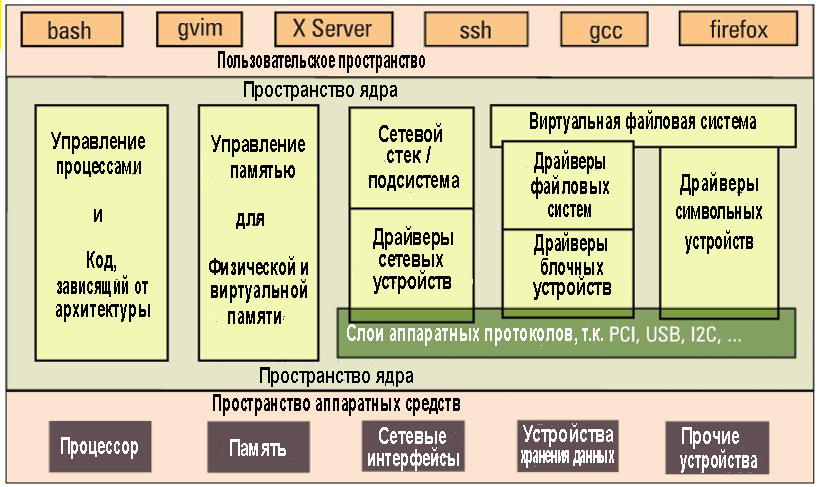
\includegraphics[width=\textwidth]{img/linux_arch}
  \caption{Пространства ОС Linux}
\end{figure}
является частью ядра. Это сделано для возможности доступа к аппаратной части.

То есть драйвер - это объектный файл, загруженный в ядро, который предоставляет набор функций для доступа к устройству из ОС. 

\subsection{Реализация драйвера}
\subsubsection{Компиляция}
Исходный код драйвера символьного устройства приведен в приложении к отчету. Структура драйвера является базовой, и может быть использована для создания драйверов для более сложных устройств.

Для получения объектного модуля, производится компиляция и  сборка исходного кода драйвера с помощью утилиты make (соответствующий makefile находится в приложении к отчету):
\lstinputlisting[caption=Лог сборки объектного файла драйвера]{sourceCode/logs/log_1.txt}
По итогу компиляции, появляется файл с раширением \textbf{.ko}. Дополнительно, с помощью команды \textbf{modinfo} можно получить информуцию о модуле.

\lstinputlisting[caption=Информация о модуле]{sourceCode/logs/log_2.txt}

\subsubsection{Встраивание в ядро}
Для загрузки модуля в ядро, используется команда \textbf{insmod} с правами суперпользователя. 
\lstinputlisting[caption=Встраивание модуля и системный лог]{sourceCode/logs/log_3.txt}
Дополнительно была выведена часть системного лога \textbf{/var/log/syslog}. Из лога видно, что были присвоены старший(250) и младший(0) номера драйвера, которые необходимы для связывания файла символьного устройства с встроенным драйвером.

Дополнительно, с помощью команды \textbf{lsmod}, можно проверить загрузку модуля.
\lstinputlisting[caption=Проверка загрузки модуля]{sourceCode/logs/log_4.txt}


\subsubsection{Создание символьного устройства}
Создать файл символьного устройства можно с помощью команды \textbf{mknod}, указав в ней старший и младший номера драйвера. 
\lstinputlisting[caption=Создание символьного устройства]{sourceCode/logs/log_5.txt}


\subsubsection{Изменение прав доступа}
Изменение прав доступа необходимо для обеспечения возможности записи и чтения файла символьного устройства. Для этого необходимо использовать команду \textbf{chmod}.
\lstinputlisting[caption=Изменение прав доступа]{sourceCode/logs/log_6.txt}


\subsubsection{Запись в файл и чтение из файла устройства}
Запись в файл символьного устройства осуществлялась с помощью команды \textbf{echo} и перенаправления потока ввода в файл символьного устройства. Чтение выполнялось с помощью команды \textbf{cat}. 
\lstinputlisting[caption=Записиь и чтение в файл символьного устройства]{sourceCode/logs/log_7.txt}

Откроем содержимое системного лога \textbf{/var/log/syslog}.
\lstinputlisting[caption=Часть системного лога]{sourceCode/logs/log_8.txt}
Из данного лога, становиться понятным, что при записи совершается: \textbf{открытие, запись, закрытие} файла, а при чтении: \textbf{открытие, чтение, закрытие} файла.


\subsubsection{Запись в файл и чтение из файла устройства (пользовательская программа)}
Также работа с символьным устройством была произведена с помощью пользовательской программы(прикреплена в приложении), суть которой заключается в выполнении команд \textbf{open, read, write, close}.
\lstinputlisting[caption=Лог пользовательской программы]{sourceCode/logs/log_9.txt}
Откроем содержимое системного лога \textbf{/var/log/syslog}.
\lstinputlisting[caption=Часть системного лога]{sourceCode/logs/log_10.txt}
Модуль сработал корректно, как и ожидалось, команды \textbf{open, read, write, close} были выполнены именно в этом порядке.


\subsubsection{Выгрузка модуля}
Для выгрузки модуля из ядра системы используется команда \textbf{rmmod} с правами суперпользователя.
\lstinputlisting[caption=Выгрузка модуля]{sourceCode/logs/log_11.txt}
В логе \textbf{/var/log/syslog} также появилась соответствующая запись.


\subsubsection{Удаление файла символьного устройства}
Для удаления файла символьного устройства используется команда \textbf{rm}.
\lstinputlisting[caption=Удаление файла символьного устройства]{sourceCode/logs/log_12.txt}


\subsubsection{Приведение каталога сборки к исходному виду}
Для очистки каталога от исполняемых файлов используется сценарий \textbf{clean} из \textbf{Makefile}.
\lstinputlisting[caption=Удаление файла символьного устройства]{sourceCode/logs/log_13.txt}


\nocite{interface}
\nocite{opennet}

\clearpage
\section*{Вывод}
Итогом данной работы является:
\begin{enumerate}
\item Изучение базовой структуры драйвера для ОС Linux;
\item Анализ функционирования драйвера символьного устройства на примере простейшего драйвера;
\item Получение базовых знаний и навыков встраивания/выгрузки модулей в ядро операционной системы.
\end{enumerate}

%------------------------------------------------------------------------------

\clearpage
\addcontentsline{toc}{section}{Список литературы}
\bibliography{thesis}
\bibliographystyle{ugost2008}

\clearpage
\addcontentsline{toc}{section}{Приложения}
\setcounter{section}{0}
\section*{Приложение 1} \label{p1:1}
\textbf{Исходный код драйвера символьного устройства chardev.c}
\lstinputlisting[caption=chardev.c]{sourceCode/chardev.c}

\section*{Приложение 2} \label{p2:1}
\textbf{Makefile}
\lstinputlisting[caption=Makefile]{sourceCode/Makefile}

\section*{Приложение 3} \label{p3:1}
\textbf{Пользовательская программа для работы с символьным устройством}
\lstinputlisting[caption=userdev.c]{sourceCode/userdev.c}

%\textbf{Алгоритм по преобразованию ascii символов в их код}
%\lstinputlisting[caption=readFile.py, label={p3:readFile}, language={[x86masm]Assembler}]{sourceCode/ascii/readFile.py}
%К сожалению, в отчет не удалось прикрепить файл, где расположена "мордочка" для вывода на дисплей, из-за невозможности отображения дополнительных символов ascii, что так-же можно заметить в листинге выше.\\\\
%
%\textbf{Мультизагрузчик}
%\lstinputlisting[caption=MultiBoot.ASM, label={p3:MultiBoot}]{sourceCode/p3/MultiBoot.ASM}



\end{document}